\documentclass[a4paper]{article}
\usepackage{graphicx}
\usepackage{amsmath}
\usepackage{titlesec}
\usepackage[a4paper,margin=0.8in]{geometry}
\usepackage{float}
\usepackage{parskip}
\usepackage{caption}
 
\titleformat{\title}{\bfseries\Huge}{}{0pt}{}
 
\title{\textbf{Is Florida Getting Warmer?}}
\author{Yanfeng Wang}
\date{November 2024}
 
\begin{document}
 
\maketitle
 
\section{Introduction}
This investigation aimed to determine whether there was a gradual increase in temperatures in Key West, Florida, throughout the 20th century.

\section{Methods}
To analyze the data, temperatures were randomly reassigned to years 10,000 times. A permutation analysis was performed to compare the distribution of random correlation coefficients with the observed correlation coefficient. The proportion of random correlation coefficients exceeding the observed value was used to estimate an approximate asymptotic \textit{p}-value.

\section{Results \& Interpretation}
The histogram in Figure 1 illustrates the distribution of random correlation coefficients.

\begin{figure}[H] % Force figure to stay here
    \centering
    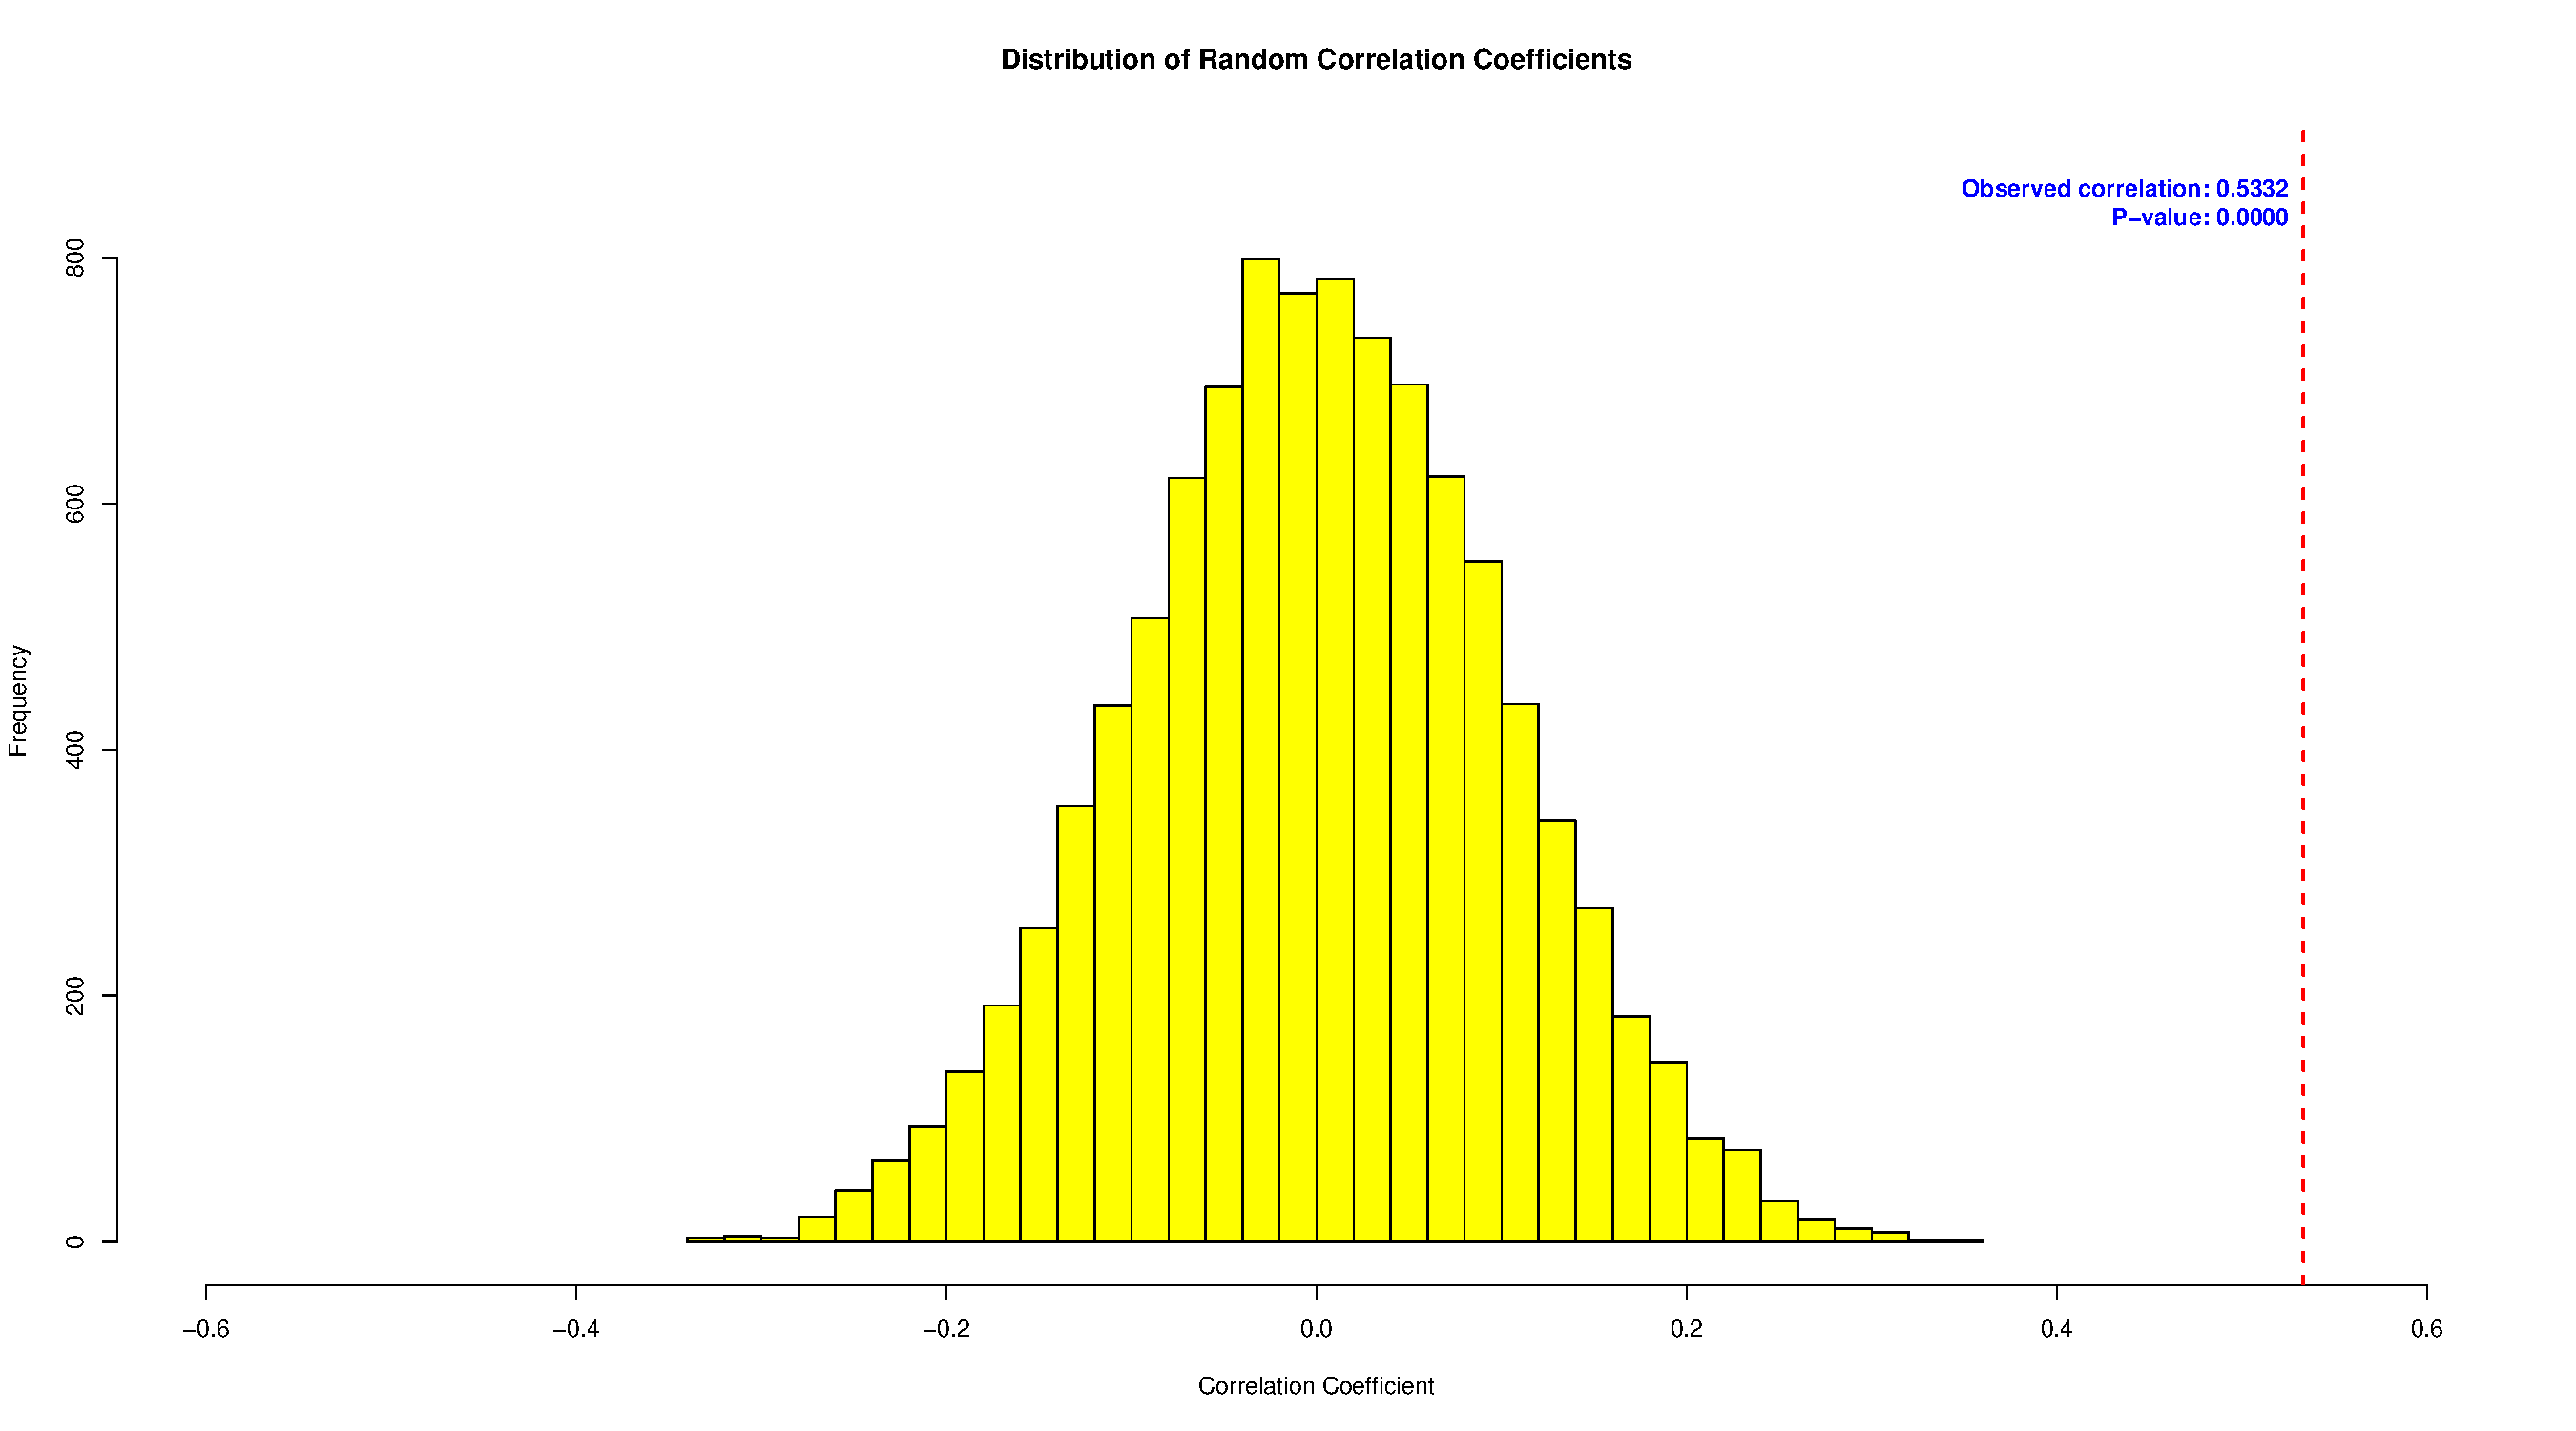
\includegraphics[width=0.9\linewidth]{../results/Florida_Correlation_Histogram.pdf}
    \captionsetup{font=footnotesize}
    \caption{Histogram of random correlation coefficients compared to the observed correlation coefficient. The red dotted line represents the observed correlation coefficient.}
    \label{fig:correlation-histogram}
\end{figure}
 
The observed correlation coefficient was approximately 0.533, with a \textit{p}-value of 0, indicating that none of the random correlation coefficients exceeded the observed value.

These findings suggest that Key West, Florida, experienced significant warming over the 20th century.
 
\end{document}